\documentclass{beamer}

\mode<presentation>{
	%\usetheme{CambridgeUS}
	%\usecolortheme{seahorse}
	\usetheme{Boadilla}
	\usecolortheme{beaver}
	\setbeamertemplate{navigation symbols}{}
}

\usepackage{graphicx}
\usepackage{booktabs}
\usepackage{algpseudocode}
\usepackage{hyperref}
\usepackage{tikz}
\usepackage[utf8]{inputenc}
\usepackage{listings}
\usepackage[export]{adjustbox}
\usepackage{aeguill}

%\setbeamertemplate{title page}[default][rounded=false]

\setbeamertemplate{title page}
{
%\vbox{}
\begingroup
\centering
\begin{beamercolorbox}[sep=8pt,center]{institute}
\usebeamerfont{institute}\insertinstitute
\end{beamercolorbox}
\vskip1em%
\begin{beamercolorbox}[sep=8pt,center]{title}
\usebeamerfont{title}\inserttitle\par%
\ifx\insertsubtitle\@empty%
\else%
\vskip0.25em%
{\usebeamerfont{subtitle}\usebeamercolor[fg]{subtitle}\insertsubtitle\par}%
\fi%
\end{beamercolorbox}%
\vfill
\begin{beamercolorbox}[sep=8pt,center]{author}
\usebeamerfont{author}\insertauthor
\end{beamercolorbox}
\vskip1em\par
\begin{beamercolorbox}[sep=8pt,center]{date}
\usebeamerfont{date}\insertdate
\end{beamercolorbox}
\endgroup
}

\setbeamertemplate{blocks}[default]
\setbeamercolor{structure}{fg=darkred}
%\setbeamercolor{block title}{bg=darkred,fg=white}
%\setbeamercolor{block body}{bg=darkgray!20!white}
\setbeamercolor{block title}{bg=darkgray!30!white}
\setbeamertemplate{enumerate items}[default]

\setbeamertemplate{part page}{
\begin{beamercolorbox}[sep=8pt,center,wd=\textwidth]{part title}
\usebeamerfont{part title}\insertpart\par
\end{beamercolorbox}
\vfill
\tableofcontents
}

%\setbeamertemplate{frametitle continuation}{(\insertcontinuationcount)}

\setbeamertemplate{headline}{\leavevmode\hbox{\begin{beamercolorbox}[wd=.5\paperwidth,ht=2.65ex,dp=1.5ex,center]{section in head/foot}\usebeamerfont{section in head/foot}\insertsectionhead\hspace*{2ex}
\end{beamercolorbox}\begin{beamercolorbox}[wd=.5\paperwidth,ht=2.65ex,dp=1.5ex,center]{subsection in head/foot}\usebeamerfont{subsection in head/foot}\hspace*{2ex}\insertsubsectionhead\end{beamercolorbox}}\vskip0pt}

\setbeamertemplate{background}{\tikz[overlay,remember picture]\node[opacity=0.08]at (current page.south east){
\includegraphics[width=10cm]{figures/unibo_logo.jpg}};}

\newcommand{\tcc}[1]{\textcolor{darkred}{#1}}

\newcommand{\codeA}[1]{\texttt{#1}}
\newcommand{\codeB}[1]{\texttt{\textcolor{darkred}{#1}}}

\newcommand{\link}[1]{{\footnotesize » \url{#1}}}
\newcommand{\bothquote}[1]{``#1''}

\definecolor{mygreen}{rgb}{0,0.6,0}
\definecolor{mygray}{rgb}{0.5,0.5,0.5}
\definecolor{mymauve}{rgb}{0.58,0,0.82}
\definecolor{maroon}{rgb}{0.5,0,0}
\definecolor{darkgreen}{rgb}{0,0.5,0}

\lstset{
language=Java,
basicstyle=\scriptsize\ttfamily,
keywordstyle=\scriptsize\color{blue}\ttfamily,
commentstyle=\scriptsize\color{mygreen}\ttfamily,
breakatwhitespace=false,
breaklines=true,
 numbers=left,
  numberstyle=\color{mymauve},
  stringstyle=\color{mymauve},
  showstringspaces=false,
  numbers=none
}

\lstdefinelanguage{XML}
{
  basicstyle=\scriptsize\ttfamily,
  morestring=[s]{"}{"},
  morecomment=[s]{?}{?},
  morecomment=[s]{!--}{--},
  commentstyle=\color{darkgreen},
  moredelim=[s][\color{black}]{>}{<},
  moredelim=[s][\color{red}]{\ }{=},
  stringstyle=\color{blue},
  identifierstyle=\color{maroon},
  numbers=none
}

\makeatother

\AtBeginSection[]
{
  \begin{frame}
    \frametitle{Outline}
    \tableofcontents[currentsection]
  \end{frame}
}

%\AtBeginSubsection[]
%{
%  \begin{frame}
%    \frametitle{Outline}
%    \tableofcontents[currentsection,currentsubsection]
%  \end{frame}
%}

\institute[UNIBO]{\uppercase{Alma Mater Studiorum -- Università di Bologna}\\Dipartimento di Informatica -- Scienza e Ingegneria (DISI)\\C.d.S. in Ingegneria e Scienze Informatiche, Campus di Cesena}

\author[A. Marfoglia]{Alberto Marfoglia\\\scriptsize\texttt{alberto.marfoglia2@unibo.it}}


\title[Android -- 2A -- Tools]{Android Programing}
\subtitle{Android SDK, Tools and Android Studio IDE}

\date[ver. 1.0 (20220505)]{Embedded Systems and Internet of Things\\A.A. 2021 -- 2022}

\begin{document}

  \begin{frame}
    \titlepage
  \end{frame}

  \newcommand\blfootnote[1]{%
  \begingroup
  \renewcommand\thefootnote{}\footnote{#1}%
  \addtocounter{footnote}{-1}%
  \endgroup
}

\begin{frame}{Thanks}
    \centering
    \begin{itemize}
      \item \large{Professor Angelo Croatti}
    \end{itemize}

    \blfootnote{\url{https://www.unibo.it/sitoweb/a.croatti/en}}
    \blfootnote{}
\end{frame}

  \begin{frame}
    \frametitle{Outline}
    \tableofcontents
  \end{frame}

  \section{Android SDK}

  \begin{frame}{Android SDK}
    \begin{columns}[c]
      \column{0.5\textwidth}
        \begin{itemize}\itemsep12pt
          \item It contains the Android Framework, the Native libraries and all
          the tools to support the development of Android App. 
          \item Using the \tcc{Android SDK Manager}, you can update the SDK,
          download add-ons or extras. 
        \begin{itemize}
          \item The components management is based on the API level.
        \end{itemize}
        \end{itemize}
      \column{0.5\textwidth}
      \begin{figure}
      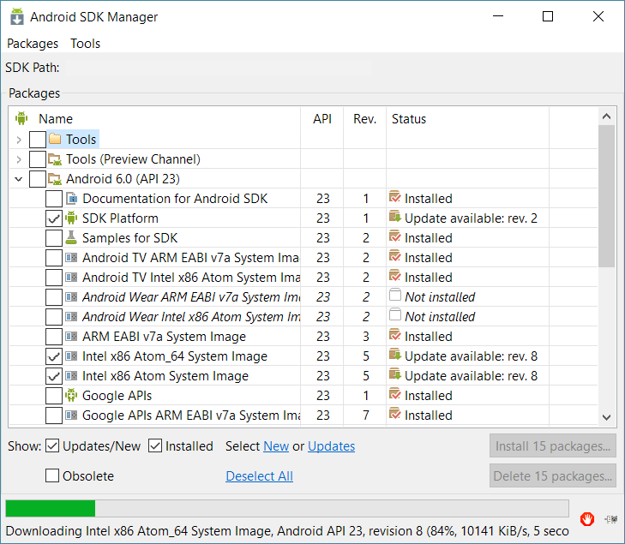
\includegraphics[width=1\linewidth]{figures/sdk-manager.png}
      \end{figure}
    \end{columns}
  \end{frame}

  \subsection{ADB}

    \begin{frame}{Android Device Bridge (adb)}
      \begin{itemize}
        \item SDK tool essential for the effective development of Android
        applications.
        \begin{itemize}
          \item It allows you to communicate with the emulator instance or with a
          physical device connected to the development environment (IDE).
        \end{itemize}
        \item Composed of 3 fundamental components.
        \begin{itemize}
          \item \tcc{client}: it runs on the same machine on which the
          application is developed and we can interact with it.
          \item \tcc{server}: it runs as a background process on the machine on
          which the application is developed, which interacts with the device
          (real or emulated).
          \item \tcc{demon}: it runs as a background process on the device (real
          or emulated). 
        \end{itemize}
        \item It can be used stand-alone or through the IDE.
      \end{itemize}
      \link{https://developer.android.com/studio/command-line/adb}
    \end{frame}

  \subsection{DDMS}

  \begin{frame}{Android DDMS}
    \begin{itemize}
      \item It provides tools for monitoring and interacting with applications
      running on an Android device (real or emulated) connected to the IDE.
      \begin{itemize}
        \item it allows to obtain the list of connected devices and related
        applications. 
      \end{itemize}
      \item Essentials for debugging.
      \item For each application it allows you to:
      \begin{itemize}
        \item Obtain all the information on the execution environment (the
        related VM)
        \item Get information about active threads (state dumping)
        \item Explore the file system (the accessible portion)
        \item Capture screenshot and get dynamic information about UI
        components. 
        \item Analyze logging flows (tool \tcc{LogCat}).
      \end{itemize}
    \end{itemize}
  \end{frame}

  \subsection{Logging}
    \begin{frame}[fragile,allowframebreaks]{Logging in Android}
      \begin{itemize}\itemsep10pt
        \item The \tcc{LogCat} tool allows you to analyze the logging flows of any
        device connected to the IDE (real or simulated) and those of a specific
        running application.
        \item In the source code, you can instruct the system to add messages to
        the logging stream.
        \item You can refer to the \codeB{android.util.Log} class, specifically
        the following static methods: 
      \begin{itemize}
      \item \codeB{Log.v(String tag, String message)} -- VERBOSE Level
      \item \codeB{Log.d(String tag, String message)} -- DEBUG Level
      \item \codeB{Log.i(String tag, String message)} -- INFO Level
      \item \codeB{Log.w(String tag, String message)} -- WARNING Level
      \item \codeB{Log.e(String tag, String message)} -- ERROR Level
    \end{itemize}
  \end{itemize}

  \begin{exampleblock}{Example - Adding a message to the Logging flow}
    \begin{lstlisting}[language=Java]
  Log.d(C.LOG_TAG, "My message content");

  /* ... */

  public class C {
    public static final String LOG_TAG = "MyAppTag";
  }
    \end{lstlisting}
  \end{exampleblock}

  \begin{itemize}\itemsep10pt
    \item The TAG can be useful for filtering the logging flow and tracing only
    the messages of interest.
    \item Note: If in Android you try to access Java StdOut (eg through
    \codeB{System.out.println (String msg))} the message is redirected to the
    logging stream, without tags, with VERBOSE level.
  \end{itemize}
  \end{frame}

\section{Android IDE}

%\begin{frame}{Ambienti di Sviluppo (IDE) per Progetti Android}
%\begin{itemize}\itemsep10pt
%\item \textbf{Android Studio}
%\begin{itemize}
%\item IDE ufficiale per lo sviluppo di Android App
%\end{itemize}
%\item Eclipse
%\begin{itemize}
%\item Supporto allo sviluppo di Android App tramite l'\tcc{ADT Eclipse Plugin} (non più supportato da Google)
%\item Disponibile una versione di Eclipse pre-configurata per Android (\tcc{Eclipse for Android Developers})
%\end{itemize}
%\item \dots
%\end{itemize}
%\vfill
%\link{https://developer.android.com/studio/}
%\end{frame}

\subsection{Android Studio}

  \begin{frame}[allowframebreaks]{Android Studio}
  \begin{itemize}\itemsep10pt
    \item Official IDE for Android App development
    \begin{itemize}
      \item Built as an extension of the \tcc{IntelliJ IDEA}
      \item Available for free (Apache 2.0 license) for all platforms (Windows,
      Mac, Linux)
      \item \link{https://developer.android.com/studio/}
    \end{itemize}
    \item Build System based on \tcc{Gradle} 
    \begin{itemize}
      \item  \url{https://gradle.org/}
    \end{itemize}
      \item It supports the \tcc{Instant Run}
      \item Integrated management of \tcc{GitHub} repositories
      \item Quick access to \tcc{Google Cloud Platform} tools
    \end{itemize}
    \begin{figure}
      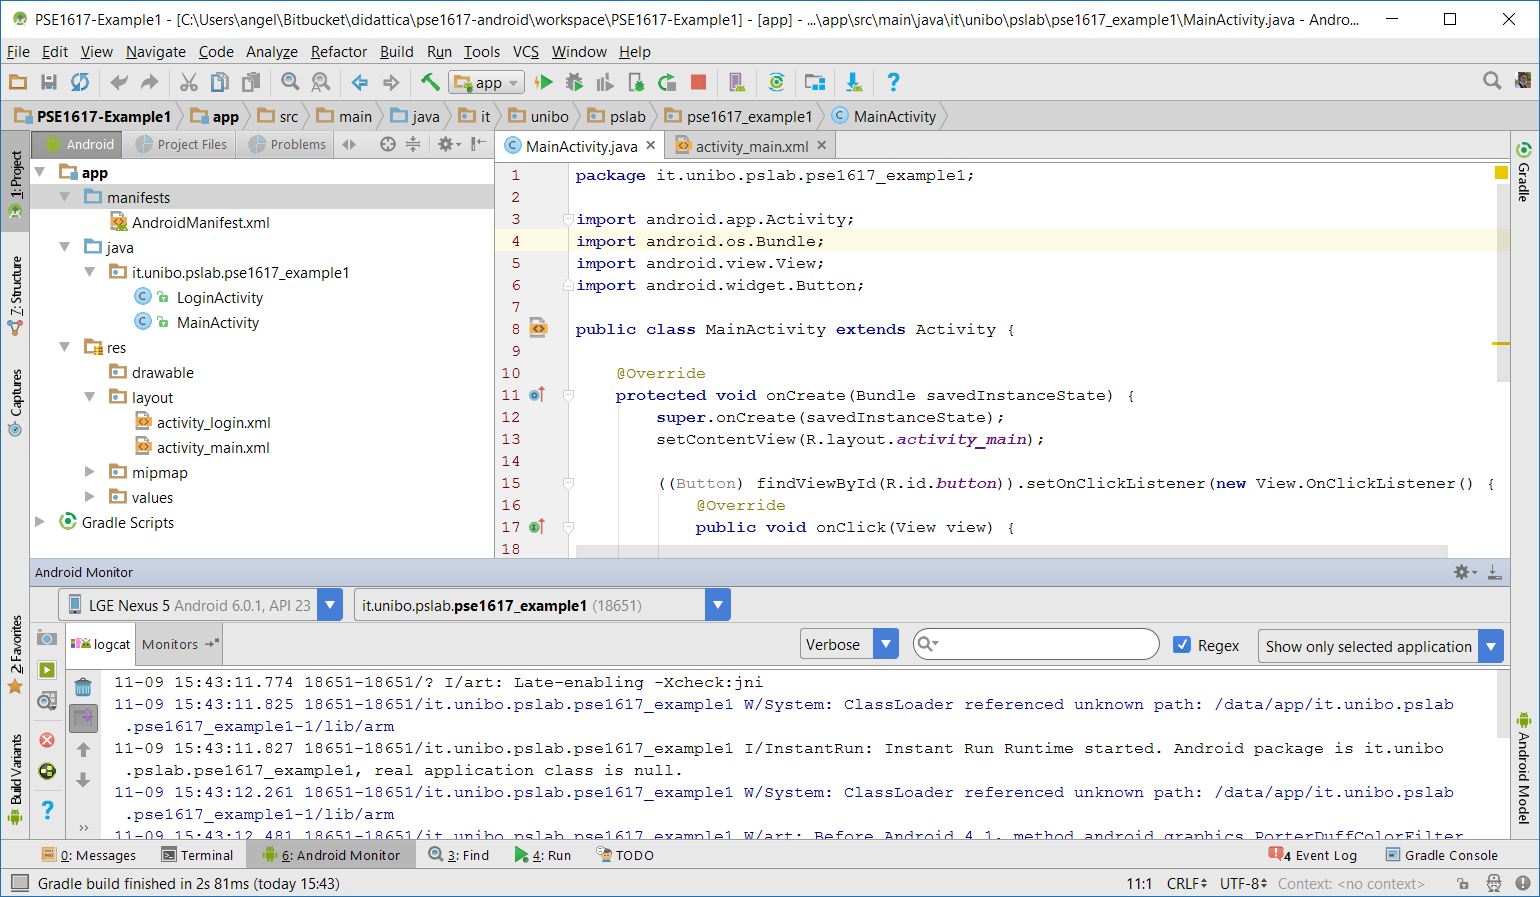
\includegraphics[width=1\linewidth]{figures/android-studio-screenshot.png}
    \end{figure}
  \end{frame}

  \begin{frame}{Android Manifest and Gradle Building}
    \begin{itemize}
      \item In Android Studio, some application-related declarations have been
      moved from the Manifest file to the \tcc{build.gradle} file in order to
      facilitate the building process.
      \begin{figure}
        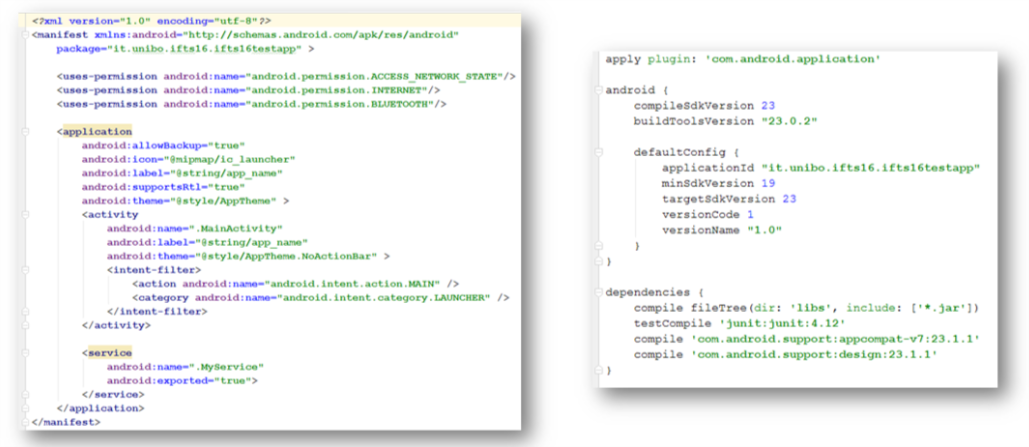
\includegraphics[width=1\linewidth]{figures/manifest-1.png}
      \end{figure}
    \end{itemize}
  \end{frame}

  \begin{frame}[fragile]{Supporto a Java 8 in Android Studio}
    \begin{itemize}
      \item To enable Java 8 feature support in Android Studio it is necessary to
      set the appropriate \tcc{compileOptions} in the \texttt{build.gradle} file
      of the project:
      \begin{lstlisting}[language=Java]
      android {
        ...
        compileOptions {
          sourceCompatibility JavaVersion.VERSION_1_8
          targetCompatibility JavaVersion.VERSION_1_8
        }
      }
      \end{lstlisting}
      \item From the UI: File $>$ Project Structure\dots $>$ (module) $>$ set
      \emph{sourceCompatibility} and \emph{targetCompatibility}
    \end{itemize}
  \end{frame}


\subsection{AVD}

  \begin{frame}{Android Virtual Device (AVD)}
    \begin{itemize}\itemsep10pt
      \item It constitutes an emulator for Android-based devices (smartphones/tables)
      \begin{itemize}
        \item You can create emulator capable of simulating most of the HW and SW
        features of any real Android-based device 
      \end{itemize}
      \item Android applications can be run (and debugged) on the emulator
      without using a physical device
      \begin{itemize}
        \item Not all characteristics of a physical device can be emulated (e.g.
        access to sensors, communication via bluetooth ,...)
      \end{itemize}
      \item In Android Studio, emulators can be created and used using the
      \tcc{AVD Manager} tool
      \begin{itemize}
        \item DDMS treats applications running on an AVD in the same way as
        those running on a physical device.
      \end{itemize}
    \end{itemize}
  \end{frame}

  \begin{frame}[allowframebreaks]{AVD Creation}
    \begin{enumerate}
      \item (in Android Studio) Menù Tools > Android > AVD Manager
      \item Click on \bothquote{Create Virtual Device...}
      \begin{figure}
        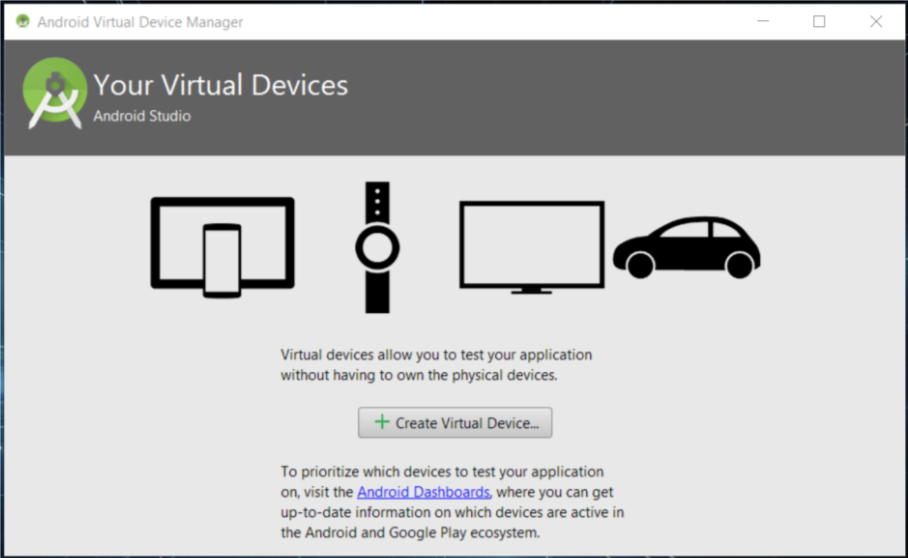
\includegraphics[width=0.8\linewidth]{figures/avd-1.png}
      \end{figure}
      \item Choose the reference hardware to be emulated
      \begin{figure}
        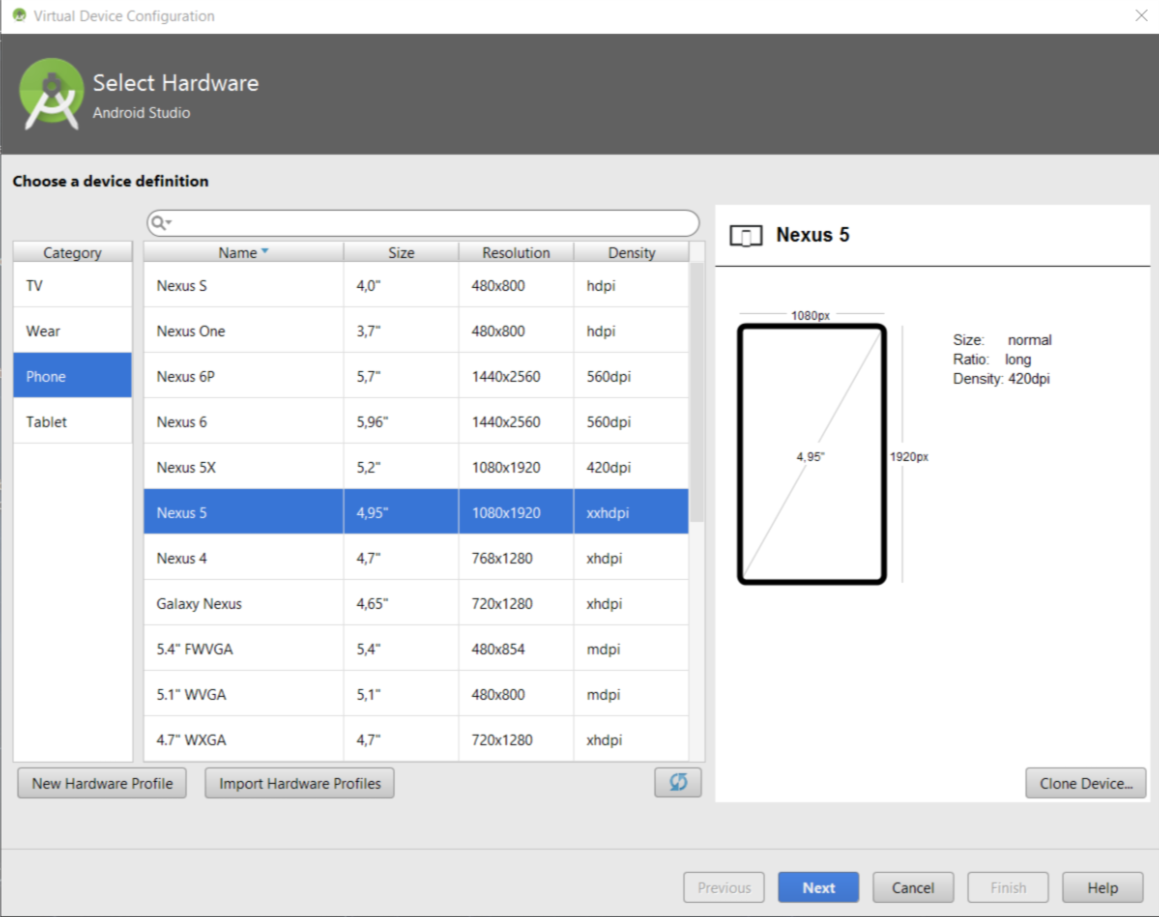
\includegraphics[width=0.7\linewidth]{figures/avd-2.png}
      \end{figure}
        \item Select the system image to be associated to the emulator
      \begin{itemize}
        \item Prefer the system images proposed in the “Recommended” section,
        which refer to system images based on Google APIs. 
        \item They can be updated/downloaded via the Android SDK Manager
      \end{itemize}
      \begin{figure}
        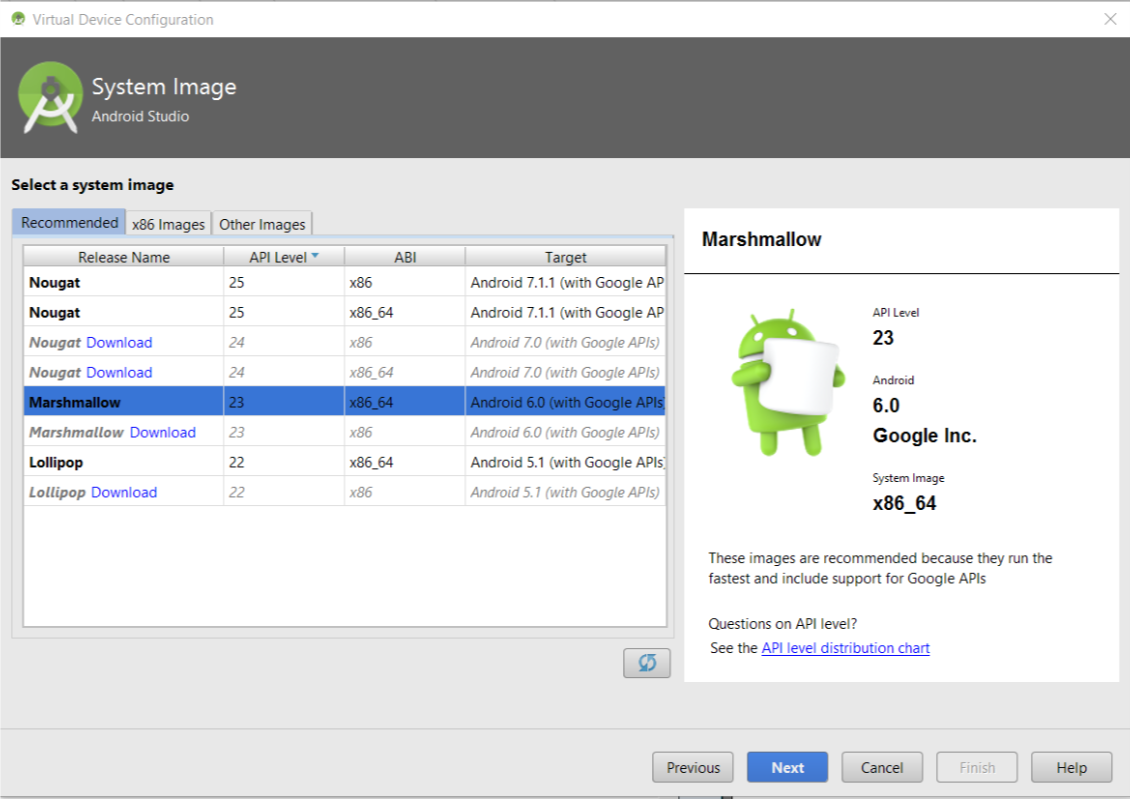
\includegraphics[width=0.8\linewidth]{figures/avd-3.png}
      \end{figure}
      \item Associate a name to the emulator and configure the advanced settings
      (\bothquote{Show Advanced Settings})
      \begin{figure}
        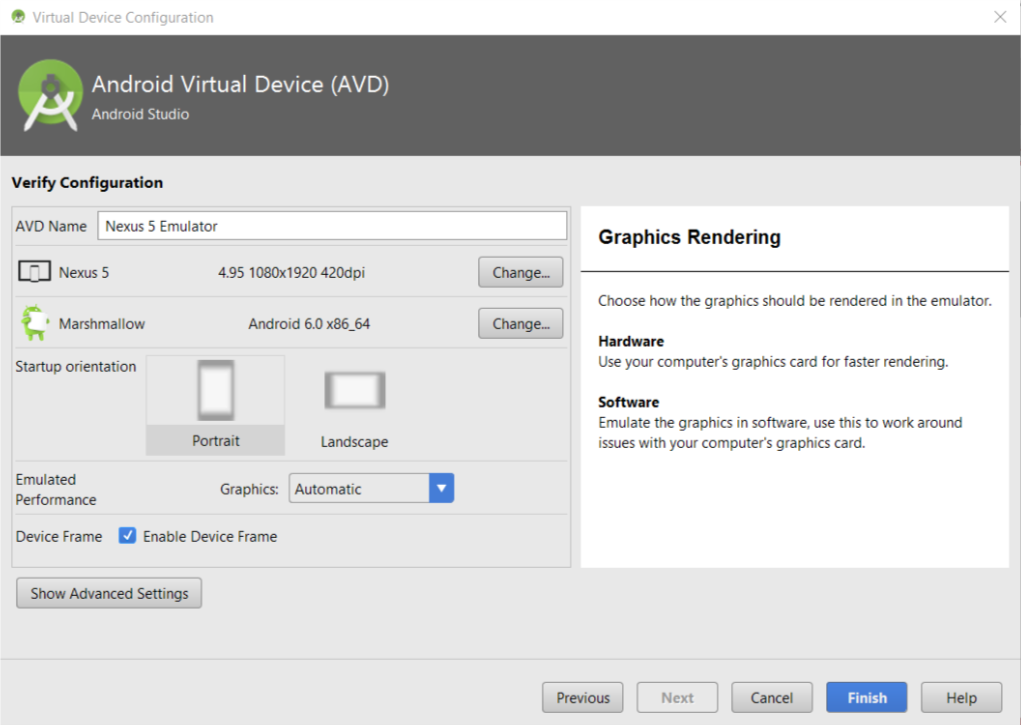
\includegraphics[width=0.75\linewidth]{figures/avd-4.png}
      \end{figure}
      \item Advanced Settings
      \begin{itemize}\itemsep10pt
        \item \tcc{Emulated Performance}: specifies whether or not to use GPU
        support (if any). We tend to leave the setting on \bothquote{Automatic}.
        \item \tcc{Camera}: a webcam installed in the system can be associated
        with the emulator, to be used as a camera for the emulator.
        \item \tcc{Memory and Storage}: it allows you to specify the amount of
        RAM to reserve for the emulator, the amount of internal storage provided
        for the emulated device and, possibly, the use of an emulated SDCard
        attached to a file in the guest file system.
        \item \tcc{Device Frame}: it allows you to customize the emulator skin. 
        \item \tcc{Keyboard}: Enables the use of the hardware keyboard connected
        to the guest system inside the emulator. 
      \end{itemize}
      \begin{figure}
      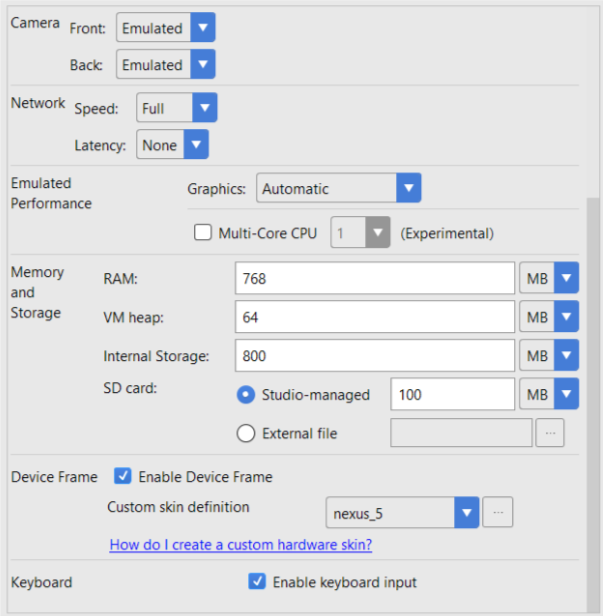
\includegraphics[width=0.65\linewidth]{figures/avd-5.png}
      \end{figure}
    \end{enumerate}
  \end{frame}

  \begin{frame}[allowframebreaks]{AVD Startup}
    \begin{itemize}
      \item At the end of the creation of the emulator, it's possible to start
      the AVD through the Launch button.
      \begin{itemize}
        \item The complete startup of the emulator can take up to a few minutes
        (times depend on the performance of the guest hardware and on whether or
        not to use the GPU support) 
      \end{itemize}
    \end{itemize}
    \begin{figure}
      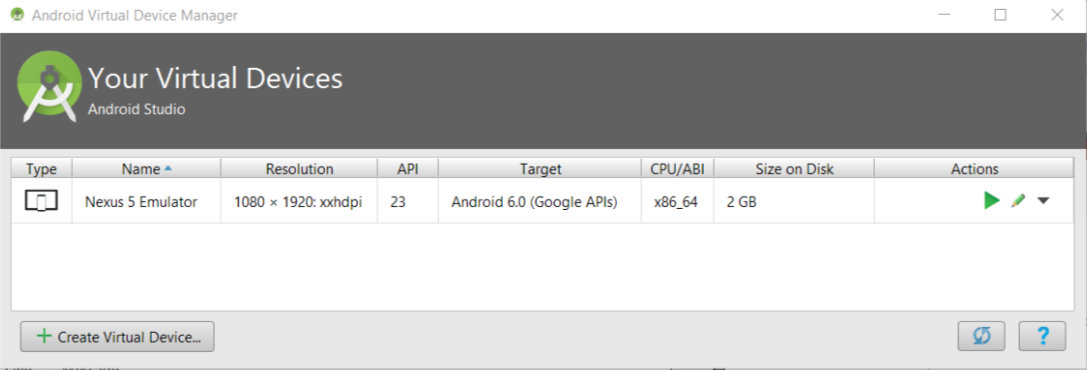
\includegraphics[width=1\linewidth]{figures/avd-6.png}
    \end{figure}

    \begin{columns}[c,onlytextwidth]
      \column{0.3\textwidth}
        \centering \tcc{-- NOTE --}\\\emph{The AVD Manager window mustn't be
        closed before the emulator is fully started!}
      \column{0.7\textwidth}
      \begin{figure}
        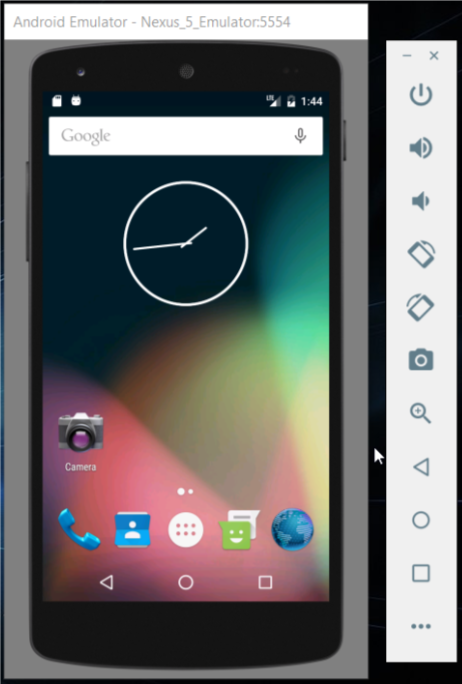
\includegraphics[width=0.55\linewidth]{figures/avd-7.png}
      \end{figure}
    \end{columns}
  \end{frame}

  \begin{frame}[allowframebreaks]{AVD Extended Controls}
    \begin{itemize}
      \item The emulator allows you to simulate the values of some sensors,
      geographic location (GPS), battery and network status.
      \item It also allows you to simulate receiving calls and sending SMS to
      the device.
      \item To access these controls, once the emulator is started, click on the
      \bothquote{More} button, the last one offered by the emulator's sidebar. 
    \end{itemize}
    \begin{figure}
      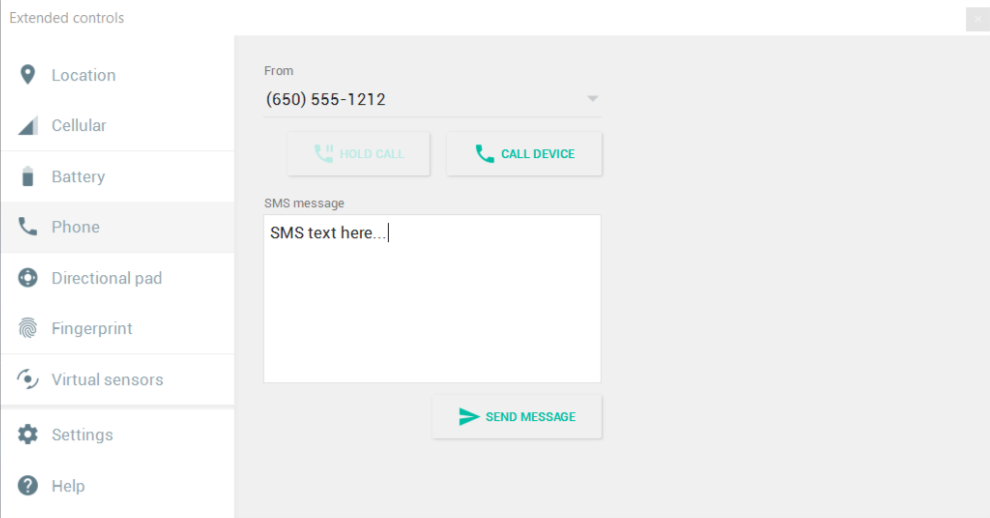
\includegraphics[width=1\linewidth]{figures/avd-8.png}
    \end{figure}
  \end{frame}

  \begin{frame}{Use of Physical Devices during development}
    \begin{itemize}\itemsep10pt
      \item A physical device on which to run the applications under development
      can be connected via USB to Android Studio. 
      \begin{enumerate}
        \item Enable developer options on the device. 
        \item In \bothquote{Developer Options}, enable USB debugging.
        \item Accept the source (PC) fingerprint at the first run of the
        application on the physical device.  
      \end{enumerate}
    \end{itemize}
  \end{frame}

\section*{References}
%-----------------------
%--- ONLINE RESURCES ---
%-----------------------

\begin{frame}{References - Online Resources}
\begin{thebibliography}{99}
\setbeamertemplate{bibliography item}[online]

\bibitem{adAPIguide} Android Developers - Guide
\newblock \link{https://developer.android.com/guide/}

\bibitem{adAPIreference} Android Developers - API Reference
\newblock \link{https://developer.android.com/reference/}

\bibitem{adTraining} Android Developers - Samples
\newblock \link{https://developer.android.com/samples/}

\bibitem{adTraining} Android Developers - Design \& Quality
\newblock \link{https://developer.android.com/design/}

\end{thebibliography}
\end{frame}

%-----------------------
%--- BOOKS -------------
%-----------------------

%\begin{frame}{Riferimenti - Libri}
%\begin{thebibliography}{99}
%\setbeamertemplate{bibliography item}[book]
%
%\bibitem{Mednieks11} Zigurd Mednieks, Laird Dornin, G. Blake Meike, Masumi Nakamura
%\newblock \emph{Programming Android}
%\newblock O'Reilly, 2011
%
%\bibitem{Haseman13} Chris Haseman, Kevin Grant
%\newblock \emph{Beginning Android Programming: Develop and Design}
%\newblock Peachpit Press, 2013
%
%\bibitem{Schwarz13} Ronan Schwarz, Phil Dutson, James Steele, Nelson To
%\newblock \emph{The Android Developer's Cookbook : Building Applications with the Android SDK}
%\newblock Addison-Wesley, 2013 
%
%\bibitem{Neil14} Theresa Neil
%\newblock \emph{Mobile Design Pattern Gallery: UI Patterns for Smartphone App}
%\newblock O'Relly, Second Edition, 2014
%\end{thebibliography}
%\end{frame}

\end{document}
